\chapter{涡量动力学}

\intro{涡量——速度场的旋度——是流体力学中最基本的场量之一。如果说压力是流动的标量势，那么涡量就是流动的矢量核。Kuchenemann曾说：涡量是流体运动的肌肉与骨骼。}

\section{涡量的基本性质}

\subsection{涡量的定义与运动学}

速度场的旋度定义为涡量：

\begin{myformula}
    \boldsymbol{\omega} = \nabla\times\mathbf{u}
\end{myformula}

在Cartesian坐标系中，涡量分量为 $\omega_i = \varepsilon_{ijk}\frac{\partial u_k}{\partial x_j}$，其中 $\varepsilon_{ijk}$ 为Levi-Civita置换符号。涡量的大小等于流体微团刚体旋转角速度的两倍：$\boldsymbol{\omega} = 2\boldsymbol{\Omega}$。

涡量与速度场之间存在运动学关系。已知涡量场时，在适当的边界条件下可唯一地确定速度场（Biot-Savart定律）：

\begin{myformula}
    \mathbf{u}(\mathbf{x}) = \frac{1}{4\pi}\int \frac{\boldsymbol{\omega}(\mathbf{x}')\times(\mathbf{x}-\mathbf{x}')}{|\mathbf{x}-\mathbf{x}'|^{3}}\,d^{3}\mathbf{x}' + \nabla\phi
\end{myformula}

其中 $\phi$ 为满足不可压缩条件的调和函数。对于无界区域中的局部涡量分布，可取 $\phi=0$。

\begin{mydefinition}{有旋流动与无旋流动}
若 $\boldsymbol{\omega} \equiv \mathbf{0}$，则流动为无旋的，速度场可表示为标量势的梯度 $\mathbf{u}=\nabla\phi$，且有 $\nabla^{2}\phi = 0$。若 $\boldsymbol{\omega}\neq\mathbf{0}$，则流动为有旋的。注意：流体微团是否旋转（有旋/无旋）与迹线是否弯曲（有环流/无环流）是两个不同概念。
\end{mydefinition}

\subsection{变形率张量与涡量}

速度梯度张量可分解为对称部分（变形率张量）与反对称部分（旋转张量）：

\begin{myformula}
    \frac{\partial u_i}{\partial x_j} = e_{ij} + \Omega_{ij},\quad
    e_{ij} = \frac{1}{2}\left(\frac{\partial u_i}{\partial x_j}+\frac{\partial u_j}{\partial x_i}\right),\quad
    \Omega_{ij} = \frac{1}{2}\left(\frac{\partial u_i}{\partial x_j}-\frac{\partial u_j}{\partial x_i}\right)
\end{myformula}

反对称张量 $\Omega_{ij}$ 与涡量矢量之间存在关系：$\Omega_{ij} = -\frac{1}{2}\varepsilon_{ijk}\omega_k$，或等价地 $\omega_i = -\varepsilon_{ijk}\Omega_{jk}$。

\subsection{涡量输运方程}

对Navier-Stokes方程取旋度，消除压力梯度项（因 $\nabla\times\nabla p \equiv 0$），得到涡量输运方程：

\begin{myformula}
    \frac{D\boldsymbol{\omega}}{D t} = \boldsymbol{\omega}\cdot\nabla\mathbf{u} + \nu\nabla^{2}\boldsymbol{\omega}
\end{myformula}

展开物质导数：

\begin{myformula}
    \frac{\partial\boldsymbol{\omega}}{\partial t} + \mathbf{u}\cdot\nabla\boldsymbol{\omega} = \boldsymbol{\omega}\cdot\nabla\mathbf{u} + \nu\nabla^{2}\boldsymbol{\omega}
\end{myformula}

方程右端两项的物理意义截然不同：
\begin{itemize}
    \item $\boldsymbol{\omega}\cdot\nabla\mathbf{u}$：涡旋拉伸/倾斜项（vortex stretching/tilting）。该项在二维流动中恒为零（$\boldsymbol{\omega}\perp\nabla\mathbf{u}$），但在三维流动中是涡量生成/增强的关键机制
    \item $\nu\nabla^{2}\boldsymbol{\omega}$：涡量的粘性扩散项，使涡量在空间中扩散，在壁面处生成边界涡量
\end{itemize}

\begin{remark}
涡量输运方程的推导消除了压力，这是其最大的优势之一。压力虽不在方程中显式出现，但其作用隐含于速度场 $\mathbf{u}$ 中（通过连续性条件）。在无粘极限 $\nu\to 0$ 下，对不可压缩流体涡量方程简化为 $\frac{D\boldsymbol{\omega}}{Dt} = \boldsymbol{\omega}\cdot\nabla\mathbf{u}$。
\end{remark}

\section{涡管与环量守恒——Helmholtz涡定理}

\subsection{涡线、涡管与涡丝}

涡线是处处与当地涡量矢量相切的曲线：$d\mathbf{x}/ds = \boldsymbol{\omega}$。涡管是由通过一封闭曲线的所有涡线组成的管状区域。涡管的强度（环量）定义为通过涡管截面的涡通量：

\begin{myformula}
    \Gamma = \int_{S} \boldsymbol{\omega}\cdot\mathbf{n}\,dS = \oint_{C} \mathbf{u}\cdot d\mathbf{l}
\end{myformula}

其中 $C$ 为截面 $S$ 的边界，等号右侧为Stokes定理的应用。

\begin{figure}[H]
\centering
\begin{tikzpicture}[scale=1.3]
    \definecolor{mytube}{RGB}{50,130,200}
    \definecolor{mysurf}{RGB}{200,220,250}
    \definecolor{mycirc}{RGB}{180,50,50}
    
    \draw[mysurf, fill=mysurf!30] (0,0) ellipse (1 and 0.4);
    \draw[mytube, line width=1pt] (1,0.4) .. controls (2,1.0) and (1,2.0) .. (0.5,3.0);
    \draw[mytube, line width=1pt] (-1,0.4) .. controls (-0.5,1.0) and (-1,2.0) .. (-0.5,3.0);
    \draw[mytube, line width=1pt] (1,-0.4) .. controls (1.5,0.5) and (0.5,1.5) .. (0.3,2.6);
    \draw[mytube, line width=1pt] (-1,-0.4) .. controls (-1.0,0.5) and (-0.5,1.5) .. (-0.3,2.6);
    
    \draw[mycirc, ->, line width=1.2pt] (0.4,2.8) arc (30:330:0.3 and 0.15);
    \draw[mycirc, ->, line width=1.2pt] (0.3,0.15) arc (30:330:0.5 and 0.2);
    
    \node at (1.5,0.7) {涡管};
    \node at (0,3.5) {$\Gamma$};
    \node at (0,-0.4) {$\Gamma_1=\Gamma_2$};
\end{tikzpicture}
\caption{涡管示意图：涡管强度（环量）沿管处处相等}
\label{fig:vortex-tube}
\end{figure}

\subsection{Helmholtz涡定理}

Helmholtz（1858年）提出了关于涡运动的三个基本定理，适用于无粘、正压（密度仅为压力的函数）、保守体力的流体：

\begin{myTheorem}{Helmholtz第一定理}
沿涡管长度，涡管强度（环量）为常数，与截面位置无关。等价地，涡管不能在流体内部起始或终止——涡管必须构成闭合环，或终止于边界，或延伸至无穷远。
\end{myTheorem}

\begin{myTheorem}{Helmholtz第二定理}
涡管随流体运动。构成涡管的流体微团始终构成同一条涡管。涡管与流体一起对流。
\end{myTheorem}

\begin{myTheorem}{Helmholtz第三定理}
在所述条件下，涡管的环量沿时间保持为常数（$\frac{D\Gamma}{Dt}=0$）。注意：粘性效应和斜压效应（密度不为压力的函数时）会使环量随时间变化。
\end{myTheorem}

\subsection{Kelvin环量定理}

Kelvin环量定理从另一个角度给出了与Helmholtz第三定理等价的陈述：对随流体运动的任意物质曲线，环量 $\Gamma$ 的物质导数为零（在无粘、正压、保守力条件下）。Kelvin定理的数学表述为：

\begin{myformula}
    \frac{D\Gamma}{Dt} = \frac{D}{Dt}\oint_{C(t)}\mathbf{u}\cdot d\mathbf{l} = 0
\end{myformula}

\begin{proof}
对物质曲线的环量求物质导数，利用运动学关系和Euler方程：
\[
\frac{D}{Dt}\oint\mathbf{u}\cdot d\mathbf{l} = \oint\frac{D\mathbf{u}}{Dt}\cdot d\mathbf{l} + \oint\mathbf{u}\cdot d\mathbf{u}
\]
第二个积分 $\oint\mathbf{u}\cdot d\mathbf{u} = \oint d(|\mathbf{u}|^{2}/2) = 0$（全微分沿闭合曲线积分为零）。第一个积分中代入Euler方程 $\frac{D\mathbf{u}}{Dt} = -\frac{1}{\rho}\nabla p + \mathbf{g}$，在给定条件下 $\oint(-\frac{1}{\rho}\nabla p + \mathbf{g})\cdot d\mathbf{l} = 0$（等号来自Stokes定理和正压条件），故 $\frac{D\Gamma}{Dt}=0$。
\end{proof}

\begin{remark}
Kelvin定理不适用于真实（粘性）流体。在粘性流体中，$\frac{D\Gamma}{Dt} = \nu\oint\nabla^{2}\mathbf{u}\cdot d\mathbf{l} \neq 0$，因此粘性是环量非守恒的主要来源之一。另一个来源是斜压效应（在大气海洋科学中非常重要）。
\end{remark}

\section{涡线的拉伸与倾斜}

\subsection{涡旋拉伸的物理机制}

三维涡量输运方程中最独特的项是 $\boldsymbol{\omega}\cdot\nabla\mathbf{u}$。考虑一根涡丝，若速度场沿涡线方向有拉伸分量（$\mathbf{u}$ 在 $\boldsymbol{\omega}$ 方向上递增），则涡线被拉长。根据角动量守恒（在无粘条件下可类比为开尔文定理的推论），拉伸导致涡丝截面减小，涡量因而增大以维持环量守恒。

数学上，不可压缩NS方程中涡量的模满足：

\begin{myformula}
    \frac{D}{Dt}\left(\frac{|\boldsymbol{\omega}|^{2}}{2}\right) = \boldsymbol{\omega}\cdot e\cdot\boldsymbol{\omega} + \nu\omega_i\nabla^{2}\omega_i
\end{myformula}

其中 $e$ 为变形率张量。$\boldsymbol{\omega}\cdot e\cdot\boldsymbol{\omega} = \omega_i e_{ij} \omega_j$ 表示涡旋与变形率场的相互作用：当涡线方向与拉伸主方向一致时，该项为正，涡量放大（enstrophy production）。

\subsection{涡旋倾斜}

涡旋倾斜（vortex tilting）是指速度梯度将涡量矢量从一个方向旋转到另一个方向的过程。例如，在边界层转捩过程中，初始的展向涡量 $\omega_z$（由流向速度剖面产生）被扰动速度场的展向梯度倾斜为流向涡量 $\omega_x$ 和法向涡量 $\omega_y$（所谓 $A$ 涡或 $Lambda$ 涡），构成湍流发生的核心机制。

\subsection{二维涡动力学的简化}

二维流动中 $\mathbf{u}=(u(x,y),v(x,y),0)$，涡量仅有一个分量 $\omega = \frac{\partial v}{\partial x} - \frac{\partial u}{\partial y}$，涡量输运方程简化为标量方程：

\begin{myformula}
    \frac{D\omega}{Dt} = \nu\nabla^{2}\omega
\end{myformula}

二维流动中涡旋拉伸项恒为零（$\boldsymbol{\omega}\cdot\nabla\mathbf{u} = \omega\frac{\partial}{\partial z}\mathbf{u} = 0$）。因此，无粘二维涡量是守恒的（沿质点的 $\omega$ 不变），仅存在粘性扩散。这一性质使二维涡动力学本质上有别于三维，也是二维湍流的物理机制与三维截然不同的根本原因。

\section{二维涡动力学}

\subsection{涡量-流函数公式}

二维不可压缩流动可方便地用流函数 $\psi$ 描述（$u=\partial\psi/\partial y$，$v=-\partial\psi/\partial x$）。涡量 $\omega$ 与流函数 $\psi$ 满足Poisson方程：

\begin{myformula}
    \nabla^{2}\psi = -\omega
\end{myformula}

这提供了涡量-流函数公式：给定涡量场，求解Poisson方程得到流函数，从而获得速度场。二维涡量输运方程可写为 $\frac{\partial\omega}{\partial t} + (\mathbf{u}\cdot\nabla)\omega = \nu\nabla^{2}\omega$，构成闭环。

\subsection{点涡与点涡系}

点涡是二维涡量场的Dirac-delta分布：$\omega(\mathbf{x}) = \Gamma\delta(\mathbf{x}-\mathbf{x}_0)$，其中 $\Gamma$ 为环量。单个点涡的诱导速度为：

\begin{myformula}
    \mathbf{u}(\mathbf{x}) = \frac{\Gamma}{2\pi r}\mathbf{e}_{\theta},\quad r = |\mathbf{x}-\mathbf{x}_0|
\end{myformula}

$N$ 个点涡之间的相互作用由Kirchhoff方程描述（Hamilton系统）：

\begin{myformula}
    \Gamma_i\frac{dx_i}{dt} = \frac{\partial H}{\partial y_i},\quad
    \Gamma_i\frac{dy_i}{dt} = -\frac{\partial H}{\partial x_i}
\end{myformula}

其中 $H = -\frac{1}{4\pi}\sum_{i\neq j}\Gamma_i\Gamma_j\ln r_{ij}$ 为Hamilton函数。点涡系统是原型混沌系统：三个或更多点涡的运动一般是混沌的。

\begin{remark}
点涡模型虽简单，但揭示了理想涡运动的许多基本特征。Onsager（1949年）将统计力学方法应用于点涡系，预言了负温度状态下同号涡会聚集成大尺度涡的"涡旋凝聚"现象，与二维湍流中能量逆级串有深刻联系。
\end{remark}

\subsection{Karman涡街}

当均匀来流绕经钝体（如圆柱），在一定Re数范围内（$40 < Re < 10^{5}$ 大致），物体后方交替脱落两列旋转方向相反的涡旋，形成著名的Karman涡街。

Karman（1911年）通过线性稳定性分析证明：交错排列（staggered arrangement）的涡街相对于对称排列是稳定的，其纵向与横向间距比 $h/\ell$ 需满足 $\sinh(\pi h/\ell) = 1$，即 $h/\ell \approx 0.281$。

涡脱落的无量纲频率由Strouhal数描述：$St = f d / U_{\infty}$，其中 $f$ 为脱落频率，$d$ 为圆柱直径。$St \approx 0.21$ 在广泛的Re数范围内基本为常数。

\begin{figure}[H]
\centering
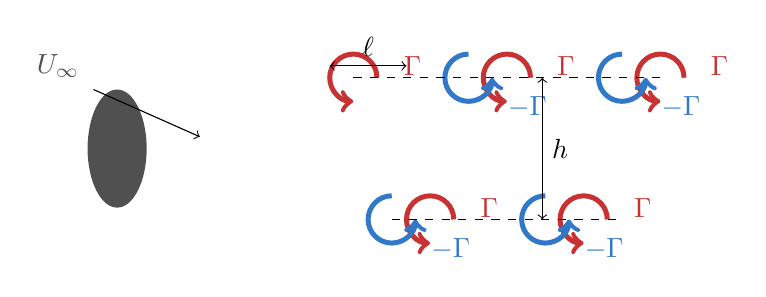
\begin{tikzpicture}[scale=1.5]
    \definecolor{myvortex1}{RGB}{200,50,50}
    \definecolor{myvortex2}{RGB}{50,120,200}
    \definecolor{mycyl}{RGB}{80,80,80}
    
    \fill[mycyl] (-1,0) ellipse (0.25 and 0.5);
    \node[mycyl] at (-1.5,0.7) {$U_{\infty}$};
    \draw[->] (-1.2,0.5) -- (-0.3,0.1);
    
    \foreach \i in {0,1,...,4} {
        \pgfmathsetmacro{\xx}{1.0 + \i*0.65}
        \pgfmathsetmacro{\yy}{0.6 * ((-1)^\i)}
        \draw[->, myvortex1, line width=1.8pt] (\xx,\yy) ++(0.2,0) arc (0:270:0.2);
        \node[myvortex1] at (\xx+0.5,\yy+0.1) {$\Gamma$};
    }
    \foreach \i in {0,1,...,3} {
        \pgfmathsetmacro{\xx}{1.325 + \i*0.65}
        \pgfmathsetmacro{\yy}{-0.6 * ((-1)^\i)}
        \draw[->, myvortex2, line width=1.8pt] (\xx,\yy+0.2) arc (90:360:0.2);
        \node[myvortex2] at (\xx+0.5,\yy-0.25) {$-\Gamma$};
    }
    
    \draw[dashed] (1.0, 0.6) -- (3.6, 0.6);
    \draw[dashed] (1.325, -0.6) -- (3.275, -0.6);
    \draw[<->] (2.6, 0.6) -- (2.6, -0.6) node[midway,right] {$h$};
    \draw[<->] (0.8, 0.7) -- (1.45, 0.7) node[midway,above] {$\ell$};
\end{tikzpicture}
\caption{Karman涡街示意：交错排列的两列反向旋转涡旋}
\label{fig:karman-vortex-street}
\end{figure}

涡街的脱落会在物体上产生交变侧向力（升力波动）。当脱落频率接近结构的固有频率时发生涡激共振（vortex-induced vibration），是塔架、桥梁、海洋立管和换热器管束发生疲劳破坏的重要原因。

\subsection{二维涡旋的合并}

两个同号涡旋在相互诱导下绕共同的质心旋转并逐渐靠近，最终合并为一个更大的涡旋。涡旋合并是二维湍流能量逆级串的基本机制——小涡合并成大涡，能量从高波数向低波数传递。合并发生的临界条件为涡间距与涡核半径之比小于某阈值。这一现象可在木星大气等地球物理流动中观测到。

\section{三维涡结构}

\subsection{马蹄涡}

在壁面湍流和边界层中，速度分布导致展向涡量 $\omega_z$ 的集中。当这些涡线在扰动下抬离壁面时，因流向速度递增而被拉伸并形成马蹄形（Horseshoe vortex，或hairpin vortex，发夹涡）。马蹄涡由两条准流向的腿部（legs）和一个抬起的头部（head）组成。

Theodorsen（1952年）首先提出了发夹涡作为壁面湍流基本结构的构想。现代DNS和实验（如PIV）已充分证实发夹涡是近壁湍流产生的核心结构，它们从壁面喷出（ejection）低速流体并诱导高速流体扫掠（sweep）壁面。

\begin{figure}[H]
\centering
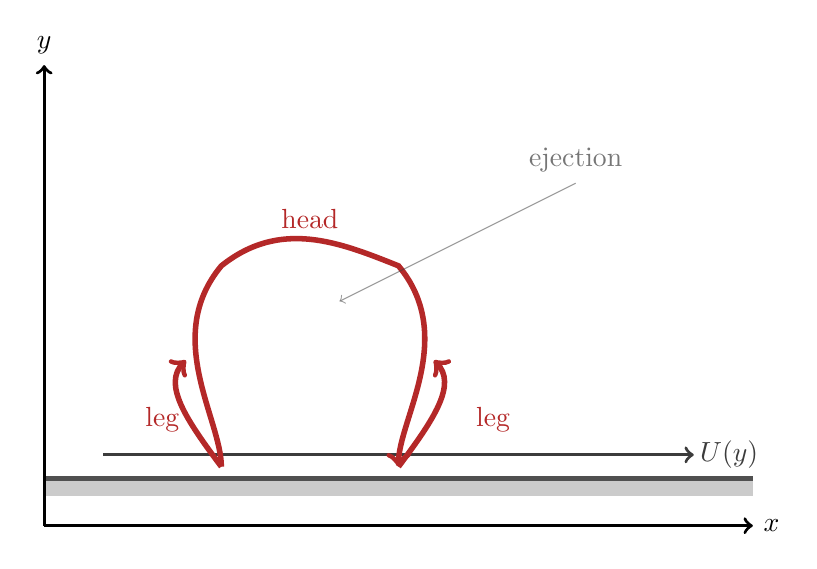
\begin{tikzpicture}[scale=1.5]
    \definecolor{mywall}{RGB}{80,80,80}
    \definecolor{myhair}{RGB}{180,40,40}
    \definecolor{myarrow}{RGB}{60,60,60}
    
    \fill[mywall!30] (0,-0.15) rectangle (6,0);
    \draw[mywall, line width=2pt] (0,0) -- (6,0);
    \draw[->, myarrow, line width=1.2pt] (0.5,0.2) -- (5.5,0.2);
    \node[myarrow] at (5.8,0.2) {$U(y)$};
    
    \draw[->, line width=1.2pt] (0,-0.4) -- (6,-0.4) node[right] {$x$};
    \draw[->, line width=1.2pt] (0,-0.4) -- (0,3.5) node[above] {$y$};
    
    \draw[myhair, line width=2pt, ->] (1.5,0.1) .. controls (1.5,0.5) and (1.0,1.2) .. (1.5,1.8)
        .. controls (2.0,2.2) and (2.5,2.0) .. (3.0,1.8)
        .. controls (3.5,1.2) and (3.0,0.5) .. (3.0,0.1);
    
    \draw[myhair, line width=2pt, ->] (1.5,0.1) .. controls (1.2,0.5) and (1.0,0.8) .. (1.2,1.0);
    \draw[myhair, line width=2pt, ->] (3.0,0.1) .. controls (3.3,0.5) and (3.5,0.8) .. (3.3,1.0);
    
    \node[myhair] at (2.25,2.2) {head};
    \node[myhair] at (1.0,0.5) {leg};
    \node[myhair] at (3.8,0.5) {leg};
    
    \draw[->, myarrow, opacity=0.5] (4.5,2.5) -- (2.5,1.5);
    \node[myarrow, opacity=0.7] at (4.5,2.7) {ejection};
\end{tikzpicture}
\caption{湍流边界层中发夹涡的示意结构：两条发夹涡的腿部指向流向，头部向上抬起}
\label{fig:hairpin-vortex}
\end{figure}

\subsection{涡环}

涡环（vortex ring）是具有环形闭合涡丝的集中涡量分布（涡核沿圆形路径）。涡环具有自诱导前进速度，使环沿垂直于环面的方向运动。轴对称涡环的自诱导速度由Saffman公式（1970年）给出：

\begin{myformula}
    U = \frac{\Gamma}{4\pi R}\left[\ln\left(\frac{8R}{a}\right) - \frac{1}{4}\right]
\end{myformula}

其中 $R$ 为环半径，$a$ 为涡核半径（$a \ll R$），$\Gamma$ 为环量。

涡环是自然界和工程中常见的涡结构：火山喷发产生的烟圈、海豚吹出的气泡圈、水下爆炸气泡的涡环效应、心脏左心室的舒张期充盈涡环等。涡环相互作用的动力学——特别是涡环的跨越（leapfrogging）现象（两个同轴涡环交替穿越对方）——是涡动力学中经典的演示实验。

\subsection{涡旋破裂}

涡旋破裂（vortex breakdown）是集中涡突然膨胀、减速并形成回流泡的现象，在三角翼前缘涡、旋风分离器和管流涡等工程问题中非常关键。其物理机制包括由于轴向减速导致的驻点形成，涡丝的不稳定性导致涡核膨胀后形成滞止泡（bubble-type）或螺旋状（spiral-type）的破裂形态。三角翼上涡旋破裂的发生决定了飞机的最大可用升力角和飞行安全边界。

\section{涡量的生成与扩散}

\subsection{壁面涡量的生成——Lighthill机制}

在无滑移壁面上，涡量是如何产生的？Lighthill（1963年）给出了经典解释：壁面处切向压力梯度驱动涡量生成。

考虑二维情形的壁面。壁面处的涡量满足：

\begin{myformula}
    \nu\frac{\partial\omega}{\partial y}\bigg|_{y=0} = \frac{1}{\rho}\frac{\partial p}{\partial x}\bigg|_{y=0}
\end{myformula}

即壁面涡量通量由壁面切向压力梯度决定。顺压力梯度（$dp/dx < 0$）使涡量从壁面向流体内部扩散（正通量），逆压力梯度（$dp/dx > 0$）反之。

更一般地，Lighthill指出三维壁面上涡量的生成率为 $\nu(\mathbf{n}\cdot\nabla)\boldsymbol{\omega}\big|_{\text{wall}} = -\mathbf{n}\times\nabla p\big|_{\text{wall}}$。涡量在壁面生成后，通过对流和扩散进入流场内部，最终由粘性耗散消除。

\subsection{涡量扩散方程}

若速度场已知，涡量扩散方程 $\frac{\partial\boldsymbol{\omega}}{\partial t} = \nu\nabla^{2}\boldsymbol{\omega}$（忽略对流项）定义了一个经典的扩散过程。基本解为Gaussian扩散核：

\begin{myformula}
    \boldsymbol{\omega}(\mathbf{x},t) = \frac{1}{(4\pi\nu t)^{3/2}}\int \boldsymbol{\omega}_0(\mathbf{x}')\exp\left(-\frac{|\mathbf{x}-\mathbf{x}'|^{2}}{4\nu t}\right)d^{3}\mathbf{x}'
\end{myformula}

在无界区域中，初始涡量分布以 $\sqrt{\nu t}$ 的速率向外扩散。

\subsection{涡量的Re数依赖性}

在 $Re \to \infty$ 的极限下（从NS方程形式上看），涡量方程的对流项主导，涡量近似为"冻结"在流体中（物质守恒）。这使得无粘涡方法成为可能。粘性效应在厚度为 $\delta_{\omega} \sim \sqrt{\nu t}$ 的涡量扩散层内重要，而在大 $Re$ 下的薄扩散层可简化为涡量的尖锐边界。

但需注意：$Re \to \infty$ 的极限是奇异的——无论Re多大，壁面处的无滑移条件始终要求涡量的生成和扩散。这一点与Prandtl边界层理论的精神完全一致。

\section{涡方法}

\subsection{涡方法的基本原理}

涡方法（Vortex Method）是计算流体力学的一类重要数值方法，其核心思想是将连续的涡量场离散为大量涡团（vortex blob、vortex particle），利用Biot-Savart定律计算速度场，追踪涡团的对流和扩散。

对于二维无粘流动，每个涡点携带环量 $\Gamma_i$，按Hamilton运动方程演化，所有非线性效应由涡系相互作用自然体现，无需直接求解NS方程的非线性项。对于三维情形，除了对流，涡团还需经历涡旋拉伸和倾斜。

含粘性时，涡量扩散可通过随机行走方法（Chorin, 1973）或粒子强度交换方法（Particle Strength Exchange, PSE）模拟。随机涡方法在每个时间步给每个涡团的位置添加Gaussian随机位移，均方根位移 $\sqrt{2\nu\Delta t}$ 精确复现了扩散方程。

\subsection{二维涡团法}

二维离散涡方法将涡量场表示为：

\begin{myformula}
    \omega(\mathbf{x},t) = \sum_{i=1}^{N} \Gamma_i\,\zeta_{\varepsilon}(|\mathbf{x}-\mathbf{x}_i|)
\end{myformula}

其中 $\zeta_{\varepsilon}$ 为光滑化涡团函数（blob function），通常取Gaussian $\zeta_{\varepsilon}(r) = \frac{1}{2\pi\varepsilon^{2}}e^{-r^{2}/2\varepsilon^{2}}$，$\varepsilon$ 为涡团光滑半径，用以避免Biout-Savart积分的奇异性。

涡团的位置演化方程为：

\begin{myformula}
    \frac{d\mathbf{x}_i}{dt} = \sum_{j\neq i} \Gamma_j\,\mathbf{K}_{\varepsilon}(\mathbf{x}_i-\mathbf{x}_j)
\end{myformula}

其中 $\mathbf{K}_{\varepsilon}$ 是正则化后的Biot-Savart核。

\subsection{涡方法的优缺点}

\textbf{优点}：
\begin{itemize}
    \item 自适应的Lagrangian描述，计算资源自动集中于涡量集中区
    \item 无网格，避免了对流项的数值耗散
    \item 远场边界条件自动满足（涡量局域化），无需人工远场边界
    \item 物理直观，直接对应涡量输运的物理过程
\end{itemize}

\textbf{缺点}：
\begin{itemize}
    \item 无滑移壁面条件的处理复杂（需在壁面生成涡量）
    \item 涡团数量随时间增加（尤其在湍流中涡量拉伸产生的极多涡片），需要重分配或涡团合并策略
    \item 粘性处理（PSE）需在散乱分布粒子上高精度离散Laplace算子
    \item 计算量随涡团数平方增长——需快速多极子方法（FMM）或树码（treecode）加速
\end{itemize}

\begin{mycode}{Python：二维点涡系统的演化}
\begin{lstlisting}[language=Python]
import numpy as np
import matplotlib.pyplot as plt
from scipy.integrate import solve_ivp

class PointVortexSystem:
    def __init__(self, positions, circulations):
        self.gamma = np.asarray(circulations)
        self.N = len(self.gamma)
        self.pos0 = np.asarray(positions).flatten()
    
    def velocity(self, pos_flat):
        x = pos_flat[0::2]; y = pos_flat[1::2]
        u = np.zeros(self.N); v = np.zeros(self.N)
        for i in range(self.N):
            for j in range(self.N):
                if i != j:
                    dx = x[i] - x[j]; dy = y[i] - y[j]
                    r2 = dx**2 + dy**2 + 1e-12
                    u[i] -= self.gamma[j] * dy / (2*np.pi * r2)
                    v[i] += self.gamma[j] * dx / (2*np.pi * r2)
        return np.column_stack([u, v]).flatten()
    
    def ode_rhs(self, t, pos_flat):
        return self.velocity(pos_flat)
    
    def simulate(self, t_max, n_steps):
        t_eval = np.linspace(0, t_max, n_steps)
        sol = solve_ivp(self.ode_rhs, [0, t_max], self.pos0,
            t_eval=t_eval, method='RK45', rtol=1e-8)
        return sol.t, sol.y

N_vortices = 6
theta = np.linspace(0, 2*np.pi, N_vortices, endpoint=False)
pos_init = np.column_stack([0.3*np.cos(theta), 0.3*np.sin(theta)])
circulations = np.ones(N_vortices) * 0.5

pvs = PointVortexSystem(pos_init, circulations)
t, y = pvs.simulate(t_max=10.0, n_steps=200)

fig, ax = plt.subplots(figsize=(8, 8))
for i in range(N_vortices):
    xi = y[2*i, :]; yi = y[2*i+1, :]
    ax.plot(xi, yi, 'o-', markersize=2, linewidth=0.5)
ax.set_xlabel('$x$'); ax.set_ylabel('$y$')
ax.set_title('Point vortex evolution')
ax.set_aspect('equal'); ax.grid(True, alpha=0.3)
plt.show()
\end{lstlisting}
\end{mycode}

\subsection{涡方法的前沿应用}

现代涡方法的发展方向包括：
\begin{itemize}
    \item 快速算法（FMM、Barnes-Hut treecode）使 $O(N^{2})$ 的计算降至 $O(N\log N)$，可处理百万级涡团
    \item 涡粒子法（Vortex Particle Method）的三维推广用于模拟湍流涡结构和混合层
    \item 耦合涡方法与边界元方法（BEM）处理复杂几何边界的涡量生成
    \item 涡方法在大涡模拟中的亚格子模型：用涡团模拟亚格子涡的输运，可精确再现背散射（backscatter）效应
\end{itemize}

\section{本章总结}

涡量动力学提供了理解流体运动的另一视角——以涡量场及其输运为核心。Helmholtz和Kelvin的环量守恒定理为无粘涡运动提供了严格框架。三维涡旋拉伸与倾斜是三维湍流区别于二维的本源机制。二维涡动力学的点涡、涡街、涡合并等经典图像构成了涡理论的基本图景。壁面上涡量的生成（Lighthill机制）和向流体内部的扩散由壁面压力梯度驱动。涡方法将这一理论框架转化为高效的Lagrangian数值工具，在漩涡主导的流动（航空尾涡、旋翼流、扑翼推进、心脏血流等）的模拟中具有独特优势。
